\chapter{Analiza, eksperymenty i trenowanie modeli uczenia maszynowego}
Dobór odpowiedniego modelu uczenia maszynowego ma duży wpływ na jakoś ostatecznej predykcji, dlatego
przeprowadzenie odpowiednich eksperymentów i sprawdzenie jakości inferencji 
(ang.~\textit{inference}) jest istotnym czynnikiem późniejszego działania aplikacji. 

\section{Analiza możliwości i wybór modelu}
Rozważono dwa sposoby przewidywania wartości VAD:

\subsection{Zamrożony model osadzeń}
Zamrożony model osadzeń zdań (ang. \textit{frozen Sentence Transformer}),
którego wektory wyjściowe trafiają do prostego regresora: regresji grzbietowej
(Ridge~\cite{Ridge}) lub modelu opartego na wzmacnianiu gradientowym drzew
decyzyjnych (XGBoost~\cite{XGBoost}).
\begin{figure}[htbp]
    \centering
    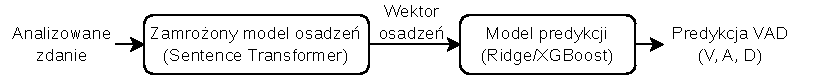
\includegraphics[width=0.9\linewidth]{figures/4/frozen_transformer.pdf}
    \caption[Potok zamrożonego modelu osadzeń]
            {Schemat potoku z zamrożonym modelem osadzeń zdań i modelem
            regresyjnym (Ridge lub XGBoost). Model osadzeń zamienia analizowane
            zdanie na wektor liczbowy, na podstawie którego regresor przewiduje
            wartości V, A i D.}
    \label{fig:frozen_pipeline}
\end{figure}


\subsection{Przedtrenowany model}
Przedtrenowany (ang. \textit{pre-trained}) model typu Transformer
dostrojony do własnego zadania (ang. \textit{fine-tuning}). Użyto modelu
DeBERTa-v3-base~\cite{he2023debertav3improvingdebertausing} firmy Microsoft.
\begin{figure}[htbp]
    \centering
    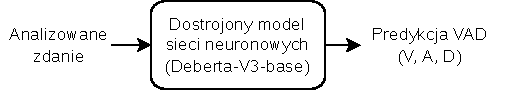
\includegraphics[width=0.7\linewidth]{figures/4/deberta_pipeline.pdf}
    \caption[Potok dostrojonego modelu DeBERTa]
            {Uproszczony schemat potoku z dostrojonym modelem DeBERTa-v3-base.
            Analizowane zdanie trafia na wejście modelu, który zwraca predykcję
            wartości V, A i D.}
    \label{fig:deberta_pipeline}
\end{figure}



\section{Badania i analiza modeli}
W tej sekcji porównano modele pod względem jakości predykcji oraz kosztu
obliczeniowego, czyli czasu trenowania i zużycia pamięci. Zestawiono ze sobą
dwa podejścia: zamrożone modele osadzeń zdań z prostym regresorem oraz
dostrojony model DeBERTa-v3-base. Celem jest wybór modelu, który najlepiej
sprawdzi się w budowanej aplikacji.


\subsection{Wstęp teoretyczny i plan eksperymentów}
\subsubsection{Środowisko testowe}
Badania wykonane były wykonywane w środowisku WSL (Windows Subsystem for Linux), komputerze o
podanej specyfikacji:
\begin{itemize}
    \item Procesor: AMD Ryzen 7 9800x3D
    \item Karta graficzna: AMD Radeon 9070xt
    \item 32GB pamięci RAM DDR5 (20GB przypisane do WSL)
\end{itemize}

Testy przeprowadzono za pomocą skryptów w języku Python, dostępnych w kodzie
źródłowym aplikacji (katalog \textit{app/ml-engine/tests})~\cite{moja_praca}.
Każdy skrypt miał prostą strukturę i odpowiadał jednemu przebiegowi potoku
przetwarzania (rys.~\ref{fig:sentence_pipeline}): wczytaniu danych, przygotowaniu
cech, treningowi, predykcji i obliczeniu metryk.

Potok dla modelu dostrajanego (rys.~\ref{fig:fine_pipeline}) wygląda nieco inaczej.
Zdania są najpierw przetwarzane przez tokenizer~\cite{wolf2020transformers,hf_transformers_docs}, 
który dzieli tekst na tokeny, zamienia je na identyfikatory liczbowe ze słownika modelu,
dodaje tokeny specjalne i wyrównuje długości zdań w paczce (ang. \textit{padding}).
Trening prowadzi klasa \textit{Trainer} z biblioteki
Transformers~\cite{wolf2020transformers,hf_trainer_docs}, która realizuje pętlę treningową,
ewaluację i zapis punktów kontrolnych. Obliczenia wykonuje biblioteka
PyTorch~\cite{paszke2019pytorch,pytorch_docs}, w tym na karcie graficznej. Hiperparametry,
takie jak współczynnik uczenia, rozmiar paczki, liczba epok czy ziarno
losowości, przekazuje się w obiekcie \textit{TrainingArguments}.


\subsubsection{Metryki porównawcze jakości modelu}
\label{sec:metrics}
Do porównania modeli wybrano pięć metryk, które razem opisują różne aspekty
jakości predykcji: wielkość błędu, zgodność kierunku zmian, zgodność wartości
oraz trafność wyznaczenia nastroju.

\paragraph{Średni błąd bezwzględny (MAE).}
Metryka określa przeciętną wielkość błędu, wyrażoną w jednostkach
etykiety
\begin{equation}
  \mathrm{MAE} = \frac{1}{N} \sum_{i=1}^{N} \lvert y_i - \hat{y}_i \rvert .
\end{equation}
Przyjmuje wartości nieujemne, a model jest tym lepszy, im wartość jest mniejsza.

\paragraph{Współczynnik korelacji Pearsona.}
Opisuje siłę liniowej zależności między predykcjami a etykietami.
W kodzie użyta została funkcjonalność biblioteki numpy, \textit{corrcoef()}~\cite{numpy_docs}. 
Wartości należą do przedziału $[-1, 1]$. Metryka jest jednak niewrażliwa na przesunięcie i skalę 
predykcji, co jest problemem przy działaniu w domenie ciągłej emocji.

\begin{figure}[p]
    \centering
    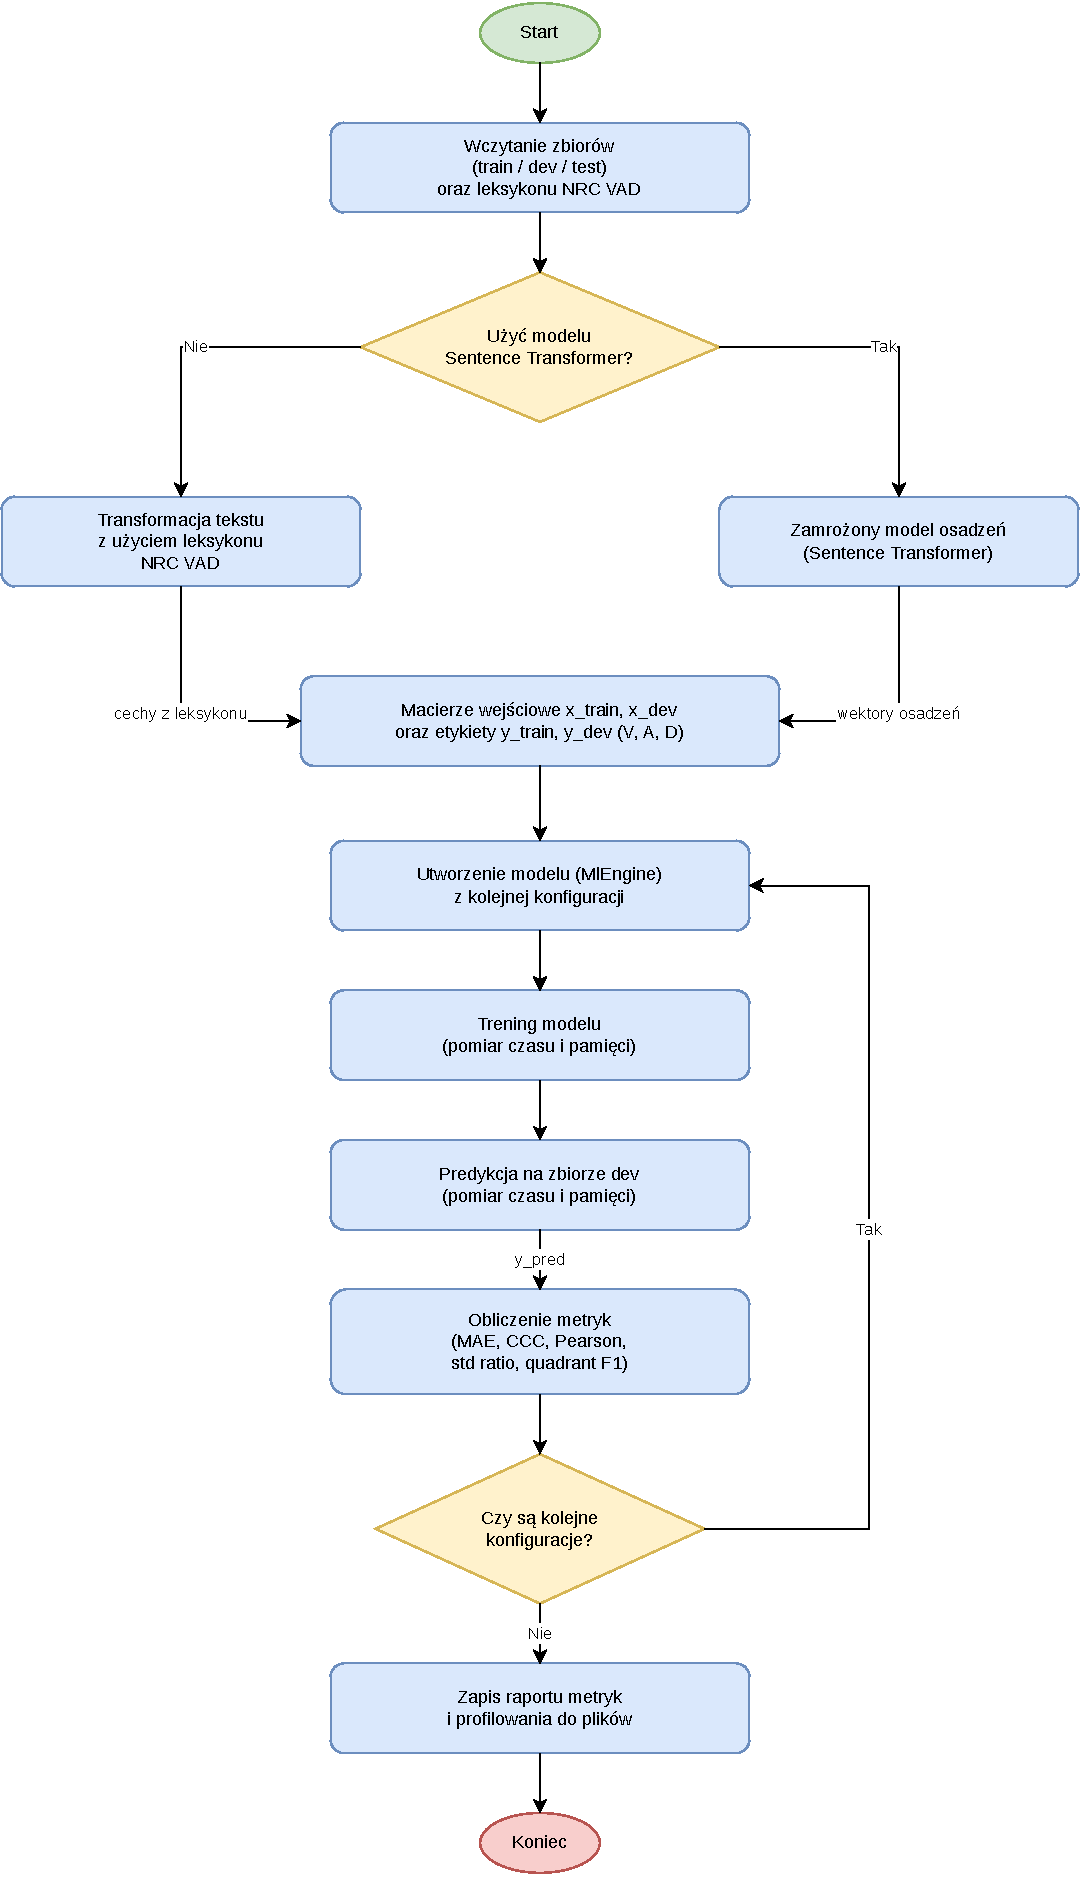
\includegraphics[height=0.9\textheight, width=\textwidth, keepaspectratio]
                    {figures/4/sentence_pipeline.pdf}
    \caption{Diagram przepływu dla skryptu testowego modeli używających macierzy wejściowych}
    \label{fig:sentence_pipeline}
\end{figure}

\begin{figure}[p]
    \centering
    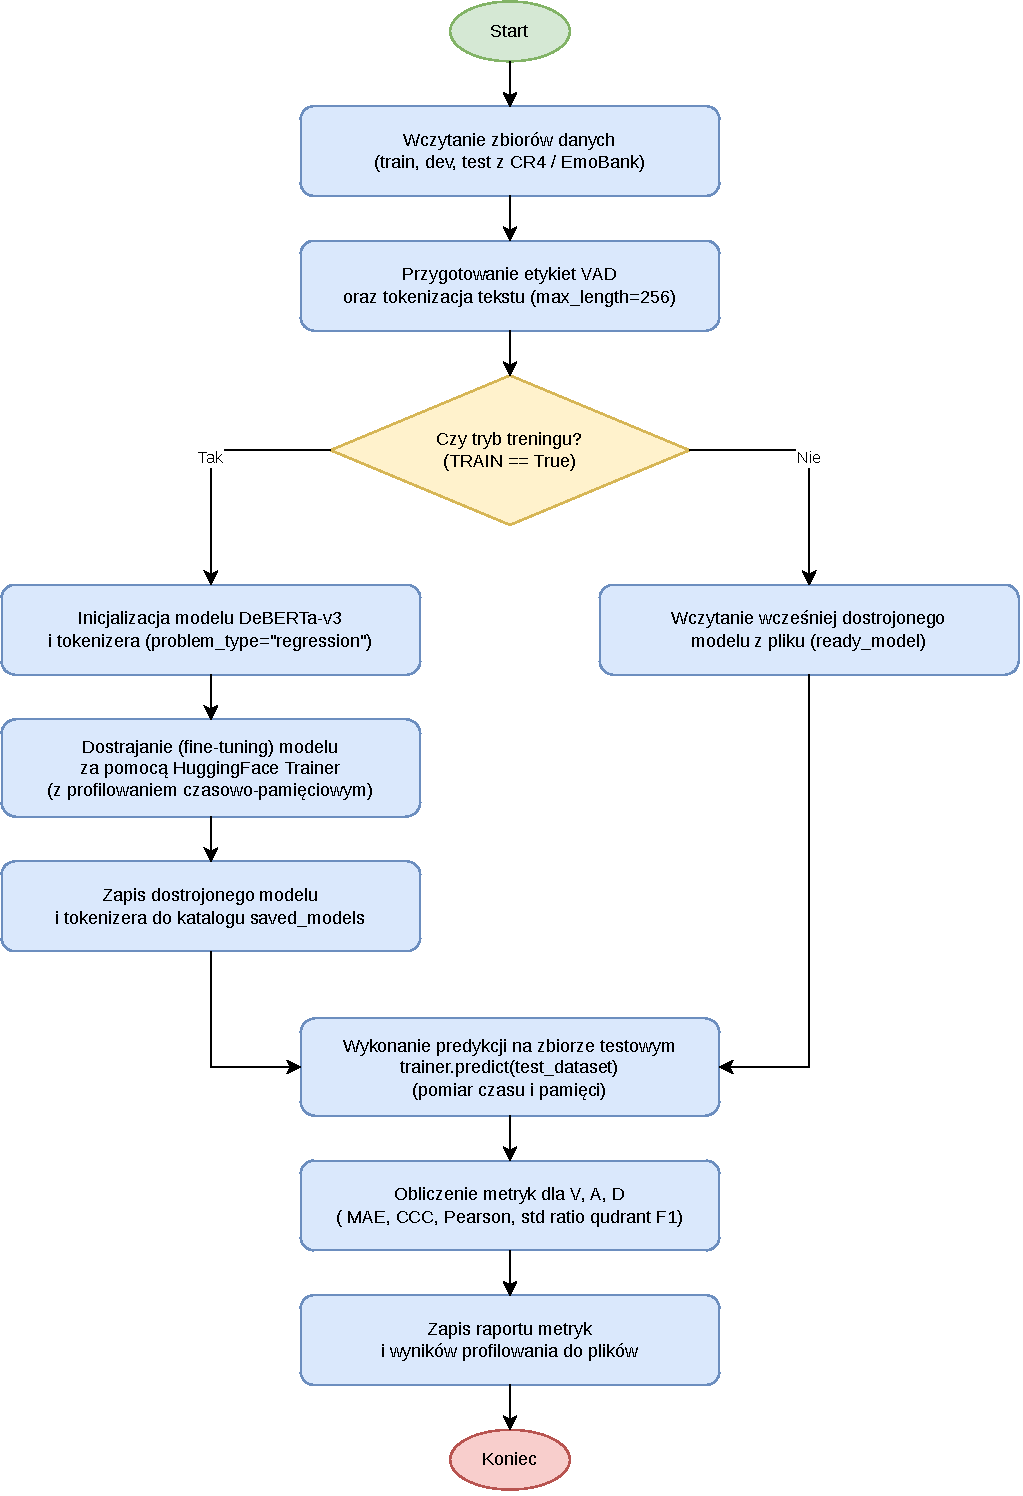
\includegraphics[height=0.9\textheight, width=\textwidth, keepaspectratio]
                    {figures/4/fine_pipeline.pdf}
    \caption{Diagram przepływu dla skryptu testowego modeli dostrajanych}
    \label{fig:fine_pipeline}
\end{figure}

\FloatBarrier
\paragraph{Współczynnik zgodności Lina (CCC).}
CCC~\cite{lin1989ccc} uwzględnia zarówno korelację, jak i różnice w średniej
oraz rozrzucie między predykcjami a etykietami:
\begin{equation}
  \mathrm{CCC} = \frac{2 r \sigma_y \sigma_{\hat{y}}}
                      {\sigma_y^2 + \sigma_{\hat{y}}^2 + (\mu_y - \mu_{\hat{y}})^2},
\end{equation}
gdzie $r$ oznacza współczynnik korelacji Pearsona, $\mu$ średnią, a $\sigma$
odchylenie standardowe. Wartość $1$ oznacza idealną zgodność ($\hat{y} = y$).
Dla $r \ge 0$ zachodzi $\mathrm{CCC} \le r$, a różnica między nimi wskazuje, jak
bardzo błędna skala lub przesunięcie obniżają jakość predykcji. Metryka jest
stosowana głównie w rozpoznawaniu emocji z mowy i obrazu (np.~\cite{valstar2016avec2016depression}).
W tej pracy użyto jej dla tekstu, ponieważ ocenia zgodność wartości, a nie tylko
ich korelację.

\paragraph{Stosunek odchyleń standardowych (std\_ratio).}
Jest to miara pomocnicza,
\begin{equation}
  \text{std\_ratio} = \frac{\sigma_{\hat{y}}}{\sigma_y},
\end{equation}
gdzie wartość bliska $1$ oznacza, że rozrzut predykcji odpowiada 
rozrzutowi etykiet. Wartość mniejsza od $1$ wskazuje na „ściśnięcie” predykcji ku średniej.

\paragraph{F1 dla ćwiartek (quadrant F1).}
Przypisuje predykcje modelu oraz ustaloną wartość ze zbioru do odpowiedniej ćwiartki za pomocą 
funkcji (lst. \ref{lst:quadrant_func})
\begin{lstlisting}[style=pythonStyle, gobble=4,
                   caption={Definicja funkcji zmieniającej ciągłą predykcję na ćwiartkę},
                   label={lst:quadrant_func}]
    def _quadrant(self, y, threshold):
        # 0: V-A-, 1: V-A+, 2: V+A-, 3: V+A+
        return (y[:, 0] > threshold).astype(int) * 2 + (y[:, 1] > threshold).astype(int)
\end{lstlisting}
Na tak uzyskanych klasach miarę $F_1$ obliczono funkcją \textit{f1\_score()}
z biblioteki scikit-learn~\cite{f1_score} z uśrednieniem makro, czyli średnią
z wartości $F_1$ obliczonych osobno dla każdej ćwiartki. Metryka ta jest
najbliższa praktycznemu zastosowaniu aplikacji, ponieważ odpowiada na pytanie,
czy dobrany nastrój mieści się w tej samej ćwiartce co nastrój tekstu.
\begin{table}[htbp]
  \centering
  \caption{Zakresy wartości i kierunek poprawy użytych metryk}
  \label{tab:metrics_summary}
  \begin{tabular}{lcc}
    \toprule
    \textbf{Metryka} & \textbf{Zakres} & \textbf{Lepszy wynik} \\
    \midrule
    MAE & $[0, \infty)$ & mniejszy \\
    Pearson & $[-1, 1]$ & większy \\
    CCC & $[-1, 1]$ & większy \\
    std\_ratio & $[0, \infty)$ & bliższy $1$ \\
    quadrant F1 & $[0, 1]$ & większy \\
    \bottomrule
  \end{tabular}
\end{table}


\subsection{Modele osadzeń}
Do porównania wybrano trzy modele osadzeń zdań dostępne w bibliotece
Sentence Transformers: all-MiniLM-L6-v2 (sekcja~\ref{sec:all_miniml}),
all-mpnet-base-v2 (sekcja~\ref{sec:all_mpnet}) oraz bge-base-en-v1.5
(sekcja~\ref{sec:bge_base}). Wybór oparto na ich popularności, otwartej
dostępności oraz zróżnicowaniu rozmiaru. Modele różnią się architekturą, danymi treningowymi, 
rozmiarem wektora wyjściowego ($384$ wymiary dla MiniLM, $768$ dla pozostałych) oraz
wydajnością (tabela~\ref{tab:sentece_trans_comp}). Wspólnym ograniczeniem
wszystkich trzech modeli jest obsługa wyłącznie języka angielskiego.

\subsubsection{all-MiniLM-L6-v2}
\label{sec:all_miniml}
Jeden z mniejszych i lżejszych modeli z rodziny 
\textit{Sentence Transformers}~\cite{all_MiniLM_L6_v2}. Model został stworzony głównie do 
transformacji pojedynczych zdań oraz krótkich paragrafów. Jako bazowy model został użyty 
\textit{nreimers/MiniLM-L6-H384-uncased}~\cite{wang2020minilm}, który następnie został 
dostrojony na miliardzie par treningowych (pary jednostek tekstowych mające pokazać modelowi 
powiązania semantyczne). Dane na których został dostrojony to głównie komentarze z portalu 
\textit{Reddit} (ok. $70\%$), dlatego domena językowa nie jest idealna dla rozwiązywanego problemu.

Model przyjmuje zdanie (do $256$ tokenów, dłuższe tekst jest ucinany) i zamienia je
na wektor $384$ liczb zmiennoprzecinkowych, który jest wejściem dla modeli
regresyjnych. Jego dużym atutem tego jest jego szybkość w porównaniu z innymi wspomnianymi 
modelami (tabela \ref{tab:sentece_trans_comp}), gdzie wykazuje niższy czas o ok. $56\%$ od mpnet 
(sekcja all-mpnet-base-v2 [\ref{sec:all_mpnet}]) i o ok. $37\%$ od bge (sekcja bge-base-en-v1.5 [\ref{sec:bge_base}]), Ma również o ok. $50\%$ niższe zużycie pamięci RAM oraz ok. $70\%$ pamięcie VRAM 
niż obydwa porównywane modele. 

\subsubsection{all-mpnet-base-v2}
\label{sec:all_mpnet}
Większy model bazowany na \textit{microsoft/mpnet-base}, podobnie do \textit{MiniLm-L6} został
dostrojony na miliardzie par treningowych~\cite{mpnet}, jednak pozwala on na wejście dłuższych form 
(384 znaki przed ucięciem), oraz na wyjściu podaje wektor $768$ liczb zmiennoprzecinkowych co 
poprawia precyzje modeli regresyjnych kosztem czasu działania (tabela~\ref{tab:sentece_trans_comp})

W eksperymentach (tabela~\ref{tab:embedding_quality_comp}) model
all-mpnet-base-v2 z regresją Ridge osiągnął CCC równe $0{,}5932$, czyli
o ok.\ $6\%$ więcej niż all-MiniLM-L6-v2 ($0{,}5579$), kosztem ponad
dwukrotnie dłuższego czasu i kilkukrotnie większego zużycia pamięci VRAM
(tabela~\ref{tab:sentece_trans_comp}). Uzyskał też najwyższą wartość
quadrant F1 spośród wszystkich zamrożonych modeli ($0{,}5014$), choć różnica
względem bge-base-en-v1.5 ($0{,}4984$) jest pomijalnie mała. W porównaniu z bge-base-en-v1.5 model 
jest wolniejszy o ok.\ $43\%$ i zużywa o ok.\ $37\%$ więcej pamięci VRAM, a mimo to osiąga
nieco niższe CCC ($0{,}5932$ wobec $0{,}6034$), więc w tym zestawieniu
nie oferuje korzyści uzasadniających wyższy koszt obliczeniowy.


\subsubsection{bge-base-en-v1.5}
\label{sec:bge_base}
Model bge-base-en-v1.5 (ang.\ \textit{BAAI General Embedding})~\cite{xiao2023cpack}
został opracowany przez Beijing Academy of Artificial Intelligence. Opiera się
na architekturze BERT i liczy około $110$ mln parametrów, a więc jest zbliżony
rozmiarem do all-mpnet-base-v2. Wektor wyjściowy ma $768$ wymiarów, a maksymalna
długość wejścia wynosi $512$ tokenów, czyli więcej niż w przypadku obu
pozostałych modeli. Trening przebiegał dwuetapowo: wstępne uczenie metodą
RetroMAE, a następnie uczenie kontrastowe na dużym zbiorze par tekstów.
Wersja $1{,}5$ ma poprawiony rozkład wartości podobieństwa w stosunku do
wersji pierwotnej. Model projektowano głównie z myślą o wyszukiwaniu
semantycznym, a nie o ocenie nastroju, dlatego jego przydatność do
przewidywania wartości VAD wymagała eksperymentalnego sprawdzenia.

W eksperymentach (tabela~\ref{tab:embedding_quality_comp}) bge-base-en-v1.5
z regresją Ridge uzyskał najlepsze wyniki spośród wszystkich zamrożonych
konfiguracji pod względem MAE ($0{,}1948$), korelacji Pearsona ($0{,}6534$)
i CCC ($0{,}6034$). CCC jest o ok.\ $8\%$ wyższe niż dla all-MiniLM-L6-v2,
jednak kosztem ok.\ $59\%$ dłuższego czasu i ok.\ $3{,}5$-krotnie większego
zużycia pamięci VRAM (tabela~\ref{tab:sentece_trans_comp}). W porównaniu
z all-mpnet-base-v2 model jest szybszy o ok.\ $30\%$ i zużywa o ok.\ $27\%$
mniej pamięci VRAM, przy podobnym zużyciu RAM, a jednocześnie osiąga wyższe
CCC ($0{,}6034$ wobec $0{,}5932$). Analiza poszczególnych wymiarów
(tabela~\ref{tab:ccc_comp}) pokazuje, że bge daje najwyższe CCC dla dominacji
($0{,}5307$) spośród trzech modeli, a dla wartościowości i pobudzenia wypada
blisko pozostałych. Najbliższy $1$ stosunek odchyleń standardowych
($0{,}7162$) uzyskał wariant z XGBoost (drzewo), jednak we wszystkich
konfiguracjach predykcje pozostają wyraźnie „ściśnięte” ku średniej.
Ze względu na najlepszą jakość przy umiarkowanym koszcie obliczeniowym
bge-base-en-v1.5 z Ridge uznano za najlepszy zamrożony model i punkt
odniesienia dla modelu dostrojonego.

\begin{table}[htbp]
    \centering
    \small
    \caption{Porównanie jakości predykcji modeli osadzeń na zbiorze CR4-NarrEmote (średnia z wymiarów V, A, D)}
    \begin{tabular}{l c c c c c}
        \toprule
        \textbf{Regresor} & \textbf{MAE} & \textbf{Pearson} & \textbf{CCC} & \textbf{std\_ratio} & \textbf{quadrant F1} \\
        \midrule
        \multicolumn{6}{l}{\textbf{all-MiniLM-L6-v2}} \\
        \hspace{1em}Ridge              & $0{,}1961$ & $0{,}6214$ & $0{,}5579$ & $0{,}6405$ & $0{,}4690$ \\
        \hspace{1em}XGBoost (regresja) & $0{,}2002$ & $0{,}6156$ & $0{,}5474$ & $0{,}6105$ & $0{,}4767$ \\
        \hspace{1em}XGBoost (drzewo)   & $0{,}2193$ & $0{,}5406$ & $0{,}5011$ & $0{,}6685$ & $0{,}4549$ \\
        \midrule
        \multicolumn{6}{l}{\textbf{all-mpnet-base-v2}} \\
        \hspace{1em}Ridge              & $0{,}1997$ & $0{,}6434$ & $0{,}5932$ & $0{,}6752$ & $\mathbf{0{,}5014}$ \\
        \hspace{1em}XGBoost (regresja) & $0{,}2013$ & $0{,}6387$ & $0{,}5820$ & $0{,}6514$ & $0{,}4992$ \\
        \hspace{1em}XGBoost (drzewo)   & $0{,}2162$ & $0{,}5834$ & $0{,}5485$ & $0{,}7043$ & $0{,}4851$ \\
        \midrule
        \multicolumn{6}{l}{\textbf{bge-base-en-v1.5}} \\
        \hspace{1em}Ridge              & $\mathbf{0{,}1948}$ & $\mathbf{0{,}6534}$ & $\mathbf{0{,}6034}$ & $0{,}6828$ & $0{,}4984$ \\
        \hspace{1em}XGBoost (regresja) & $0{,}1953$ & $0{,}6515$ & $0{,}5980$ & $0{,}6658$ & $0{,}4967$ \\
        \hspace{1em}XGBoost (drzewo)   & $0{,}2103$ & $0{,}5970$ & $0{,}5645$ & $\mathbf{0{,}7162}$ & $0{,}4932$ \\
        \bottomrule
    \end{tabular}
    \label{tab:embedding_quality_comp}
\end{table}


\FloatBarrier
\subsection{Porównanie modeli osadzeń do dostrojonego modelu}
\label{sec:deberta_theory}
DeBERTa (ang.\ \textit{Decoding-enhanced BERT with disentangled
attention})~\cite{he2021deberta} jest modelem typu Transformer rozwijającym
architekturę BERT. Jego główną innowacją jest rozdzielona uwaga (ang.\
\textit{disentangled attention}): treść każdego tokenu i jego pozycja są
reprezentowane osobnymi wektorami, a waga uwagi między tokenami zależy zarówno od
ich treści, jak i od wzajemnego położenia. Ułatwia to modelowi rozpoznawanie
zależności składniowych, takich jak zaprzeczenia, co ma znaczenie przy ocenie
nastroju zdania.

Wersja DeBERTaV3~\cite{he2023debertav3improvingdebertausing} zachowuje tę
architekturę, ale zmienia sposób wstępnego uczenia. Zamiast przewidywania
zamaskowanych tokenów zastosowano zadanie wykrywania zastąpionych tokenów (ang.\
\textit{replaced token detection})~\cite{clark2020electra}, w którym model dla
każdego tokenu zdania ocenia, czy jest oryginalny, czy podstawiony. Sygnał uczący
pochodzi wtedy ze wszystkich pozycji, a nie tylko z zamaskowanych, co zwiększa
efektywność uczenia. Dodatkowo zastosowano współdzielenie osadzeń z rozdzieleniem
gradientów (ang.\ \textit{gradient-disentangled embedding sharing}), które
eliminuje wzajemne zakłócanie się generatora i dyskryminatora podczas treningu.

Model DeBERTa-v3-base~\cite{deberta_v3_base} ma $12$ warstw, wymiar warstwy
ukrytej $768$ oraz słownik liczący $128$ tys.\ tokenów. Szkielet sieci liczy ok.\
$86$ mln parametrów, a duża warstwa osadzeń dodaje kolejne ok.\ $98$ mln, co daje
łącznie ok.\ $184$ mln parametrów. W niniejszej pracy model dostrojono
(ang.\ \textit{fine-tuning}) do przewidywania wartości V, A i D: do enkodera
dołączono głowicę regresyjną o trzech wyjściach, a uczeniu podlegała cała sieć.
W przeciwieństwie do podejścia z zamrożonym modelem osadzeń pozwala to dopasować
reprezentację tekstu do zadania, co potwierdzają wyniki w
tabeli~\ref{tab:embedding_quality_comp_deberta}.

\begin{table}[htbp]
    \centering
    \caption{Porównanie wydajności rozważanych modeli}
    \begin{tabular}{l l p{3.7cm} p{3.7cm}}
        \toprule
        \textbf{Nazwa modelu} & \textbf{Czas [s]} & \textbf{Maksymalne zużycie pamięci RAM [kB]} & \textbf{Maksymalne zużycie pamięci VRAM [kB]} \\
        \midrule
        \textbf{all-MiniLM-L6-v2}  & $15{,}93$ & $48\,874{,}57$  & $296{,}83$ \\
        \textbf{all-mpnet-base-v2} & $36{,}22$ & $100\,321{,}43$ & $1\,412{,}90$ \\
        \textbf{bge-base-en-v1.5}  & $25{,}38$ & $100\,624{,}01$ & $1\,031{,}10$ \\
        \textbf{DeBERTa-v3-base}   & $33{,}10$ & $231{,}48$      & $5\,777{,}02$ \\
        \bottomrule
    \end{tabular}
    \label{tab:sentece_trans_comp}
\end{table}

Mimo wyższego kosztu obliczeniowego, w tym większego zużycia pamięci VRAM
(tabela~\ref{tab:sentece_trans_comp}), dostrojony model DeBERTa-v3-base osiąga
wyraźnie lepszą jakość predykcji niż modele z zamrożonym osadzeniem
(tabele~\ref{tab:embedding_quality_comp_deberta} i~\ref{tab:ccc_comp}).
Przewaga widoczna jest we wszystkich pięciu metrykach uśrednionych po wymiarach
V, A i D, a największa w \textit{std\_ratio} oraz quadrant F1. Oznacza to, że
model nie tylko trafniej przewiduje wartości, ale też w mniejszym stopniu
„ściska'' predykcje ku środkowi skali, dzięki czemu częściej poprawnie wskazuje
ćwiartkę nastroju. Dla porównania, najlepszy model z zamrożonym osadzeniem
osiągnął \textit{std\_ratio} równe $0{,}7162$ i quadrant F1 równe $0{,}5014$,
a DeBERTa odpowiednio $0{,}9021$ i $0{,}6242$.

\begin{table}[htbp]
    \centering
    \small
    \caption{Porównanie jakości predykcji rozważanych modeli na zbiorze CR4-NarrEmote (średnia z wymiarów V, A, D)}
    \begin{tabular}{l c c c c c}
        \toprule
        \textbf{Metoda} & \textbf{MAE} & \textbf{Pearson} & \textbf{CCC} & \textbf{std\_ratio} & \textbf{quadrant F1} \\
        \midrule
        \multicolumn{6}{l}{\textbf{all-MiniLM-L6-v2} (zamrożony)} \\
        \hspace{1em}Ridge              & $0{,}1961$ & $0{,}6214$ & $0{,}5579$ & $0{,}6405$ & $0{,}4690$ \\
        \hspace{1em}XGBoost (regresja) & $0{,}2002$ & $0{,}6156$ & $0{,}5474$ & $0{,}6105$ & $0{,}4767$ \\
        \hspace{1em}XGBoost (drzewo)   & $0{,}2193$ & $0{,}5406$ & $0{,}5011$ & $0{,}6685$ & $0{,}4549$ \\
        \midrule
        \multicolumn{6}{l}{\textbf{all-mpnet-base-v2} (zamrożony)} \\
        \hspace{1em}Ridge              & $0{,}1997$ & $0{,}6434$ & $0{,}5932$ & $0{,}6752$ & $0{,}5014$ \\
        \hspace{1em}XGBoost (regresja) & $0{,}2013$ & $0{,}6387$ & $0{,}5820$ & $0{,}6514$ & $0{,}4992$ \\
        \hspace{1em}XGBoost (drzewo)   & $0{,}2162$ & $0{,}5834$ & $0{,}5485$ & $0{,}7043$ & $0{,}4851$ \\
        \midrule
        \multicolumn{6}{l}{\textbf{bge-base-en-v1.5} (zamrożony)} \\
        \hspace{1em}Ridge              & $0{,}1948$ & $0{,}6534$ & $0{,}6034$ & $0{,}6828$ & $0{,}4984$ \\
        \hspace{1em}XGBoost (regresja) & $0{,}1953$ & $0{,}6515$ & $0{,}5980$ & $0{,}6658$ & $0{,}4967$ \\
        \hspace{1em}XGBoost (drzewo)   & $0{,}2103$ & $0{,}5970$ & $0{,}5645$ & $0{,}7162$ & $0{,}4932$ \\
        \midrule
        \textbf{DeBERTa-v3-base} (dostrojony) & $\mathbf{0{,}1712}$ & $\mathbf{0{,}7418}$ & $\mathbf{0{,}7349}$ & $\mathbf{0{,}9021}$ & $\mathbf{0{,}6242}$ \\
        \bottomrule
    \end{tabular}
    \label{tab:embedding_quality_comp_deberta}
\end{table}

\begin{table}[htbp]
    \centering
    \small
    \caption{Współczynnik zgodności Lina (CCC) rozważanych modeli na zbiorze CR4-NarrEmote, osobno dla wymiarów V, A, D. Większa wartość oznacza lepszy wynik, pogrubiono najlepsze wyniki}
    \begin{tabular}{l c c c c}
        \toprule
        \textbf{Metoda} & \textbf{CCC V} & \textbf{CCC A} & \textbf{CCC D} & \textbf{Średnia} \\
        \midrule
        \multicolumn{5}{l}{\textbf{all-MiniLM-L6-v2} (zamrożony)} \\
        \hspace{1em}Ridge              & $\mathbf{0{,}9181}$ & $0{,}3173$ & $0{,}4383$ & $0{,}5579$ \\
        \hspace{1em}XGBoost (regresja) & $0{,}8916$ & $0{,}3307$ & $0{,}4198$ & $0{,}5474$ \\
        \hspace{1em}XGBoost (drzewo)   & $0{,}8435$ & $0{,}2878$ & $0{,}3720$ & $0{,}5011$ \\
        \midrule
        \multicolumn{5}{l}{\textbf{all-mpnet-base-v2} (zamrożony)} \\
        \hspace{1em}Ridge              & $0{,}8414$ & $0{,}4186$ & $0{,}5195$ & $0{,}5932$ \\
        \hspace{1em}XGBoost (regresja) & $0{,}8241$ & $0{,}4090$ & $0{,}5130$ & $0{,}5820$ \\
        \hspace{1em}XGBoost (drzewo)   & $0{,}7885$ & $0{,}3811$ & $0{,}4760$ & $0{,}5485$ \\
        \midrule
        \multicolumn{5}{l}{\textbf{bge-base-en-v1.5} (zamrożony)} \\
        \hspace{1em}Ridge              & $0{,}8712$ & $0{,}4084$ & $0{,}5307$ & $0{,}6034$ \\
        \hspace{1em}XGBoost (regresja) & $0{,}8597$ & $0{,}4093$ & $0{,}5249$ & $0{,}5980$ \\
        \hspace{1em}XGBoost (drzewo)   & $0{,}8278$ & $0{,}3709$ & $0{,}4948$ & $0{,}5645$ \\
        \midrule
        \textbf{DeBERTa-v3-base} (dostrojony) & $0{,}8929$ & $\mathbf{0{,}6406}$ & $\mathbf{0{,}6713}$ & $\mathbf{0{,}7349}$ \\
        \bottomrule
    \end{tabular}
    \label{tab:ccc_comp}
\end{table}

\FloatBarrier
\section{Wnioski}
Do dalszych prac wybrano dostrojony model DeBERTa-v3-base, ponieważ uzyskał
najlepsze wyniki spośród wszystkich porównywanych podejść. Jego CCC wyniosło
$0{,}7349$, wobec $0{,}6034$ dla najlepszego modelu z zamrożonym osadzeniem
(bge-base-en-v1.5 z regresją Ridge), a quadrant F1 wyniosło $0{,}6242$ wobec
$0{,}5014$. Przewaga wynika głównie z lepszego przewidywania pobudzenia
i dominacji, natomiast dla wartościowości zamrożone osadzenia radziły sobie
porównywalnie. Modele oparte wyłącznie na cechach leksykonowych okazały się
wyraźnie słabsze (najlepsze CCC: $0{,}2853$), co potwierdza, że sama emocjonalna
wartość pojedynczych słów nie wystarcza do oceny nastroju fragmentu.

Wybór wiąże się z wyższym kosztem obliczeniowym, w tym większym zużyciem pamięci
VRAM (tabela~\ref{tab:sentece_trans_comp}). Przy ciągłej analizie czytanego
tekstu w czasie rzeczywistym ma to znaczenie, dlatego w dalszych etapach należy
ograniczyć liczbę wywołań modelu, na przykład poprzez analizę dopiero po
zatrzymaniu przewijania strony oraz zapamiętywanie wyników dla już
przetworzonych fragmentów lub zmianę podejścia na analizę wstępną książki po wczytaniu przez
użytkownika i zapisu predykcji dla zdań w oddzielnym pliku, który użyty będzie do samej analizy. 
Uzasadnia to także wydzielenie modułu NLP do osobnego kontenera.

Uzyskane wyniki dają dobrą bazę pod dalsze prace, jednak nie rozwiązują
problemu w całości. Wartość quadrant F1 na poziomie $0{,}6242$ oznacza, że model
wciąż w istotnej części przypadków wskazuje niewłaściwą ćwiartkę nastroju. Samo przewidzenie 
wartości VAD jest ponadto tylko jednym z etapów doboru muzyki: kolejnym jest przypisanie
utworów do ćwiartek nastroju oraz logika decyzyjna (progowanie), która ograniczy
zbyt częste zmiany ścieżki dźwiękowej przy niepewnych predykcjach.
